%%%%%%%%%%%%%%%%%%%%%%%%%%%%%%%%%%%%%%%%%%%%%%%%%%%%%%%%%%%%%%%%%%%%%%%%%%%%%%%%
%
% LICENZA
%
% Quest'opera è stata rilasciata sotto la licenza
% Creative Commons Attribution-NonCommercial-ShareAlike 2.5 Italy.
% Per leggere una copia della licenza visita il sito web
% http://creativecommons.org/licenses/by-nc-sa/2.5/it/
% o spedisci una lettera a Creative Commons, 171 Second Street, Suite 300, San
% Francisco, California, 94105, USA.
%
% This work is licensed under the Creative Commons
% Attribution-NonCommercial-ShareAlike 3.0 Unported License. To view a copy of
% this license, visit http://creativecommons.org/licenses/by-nc-sa/3.0/ or send
% a letter to Creative Commons, 171 Second Street, Suite 300, San Francisco,
% California, 94105, USA.
%
% For info send a mail to pietro.giuffri@gmail.com
%
%%%%%%%%%%%%%%%%%%%%%%%%%%%%%%%%%%%%%%%%%%%%%%%%%%%%%%%%%%%%%%%%%%%%%%%%%%%%%%%%

\documentclass[b5paper,11pt,oneside]{guidatematica}
\ProvidesFile{guidagit.tex}[2013/07/06 v.0.2 Una guida introduttiva a Git per
progetti LaTeX]

\usepackage[os=win]{menukeys}
\usepackage{quoting,hyperref}

\hypersetup{
  pdftitle={Una guida introduttiva a Git per progetti \LaTeX},
  pdfauthor={Pietro Giuffrida, Mosè Giordano},
  breaklinks=true, % permette di spezzare i link su più righe
  bookmarksnumbered, % inserisce i numeri delle sezioni nei segnalibri
  %%% opzioni dei colori di guidatematica.cls
  colorlinks,linkcolor={blue},
  citecolor={blue!80!black},urlcolor={blue},
}

\lstset{basicstyle=\small\ttfamily,
  keywordstyle=\color{blue},
  commentstyle=\color{red},
  stringstyle=\color{purple},
  frame=lines,
  breaklines = true, % per mandare a capo le righe troppo lunghe
  breakautoindent = true, % indenta le righe spezzate
  breakindent = 30pt, % indenta le righe di 30pt
  language=bash,
  showspaces=false,
  showstringspaces=false,
  showtabs=false,
  emph={touch,mkdir,echo,rm},
  emphstyle=\color{blue},
  escapechar={£},
}

% comando per scrivere `GiT' con lo stile di `TeX', da usare nel titolo.  Ho
% copiato la definizione del comando `\TeX'.
\newcommand{\GiT}{G\kern-.1667em\lower.5ex\hbox{I}\kern-.125emT\@}

\begin{document}
\title{\GiT{} 4 \LaTeX{} \\
  Una guida introduttiva a Git per progetti \LaTeX}
\author{Pietro Giuffrida, Mosè Giordano}

\frontmatter{}
\GetFileInfo{guidagit.tex}
\date{\fileversion{} del \filedate}

\maketitle

\cleardoublepage{}
\chapter{Presentazione della guida}
\label{cha:presentazione-guida}

In questa guida mostreremo come utilizzare Git per tener traccia delle modifiche
rilevanti e delle versioni elaborate nel corso dell'elaborazione di un documento
scritto con \LaTeX, un programma di composizione tipografica di alta qualità.
Qui non si spiegherà il funzionamento di \LaTeX{}, per maggiori informazioni su
questo programma si possono consultare l'ottima guida di~\cite{pantieri:latex} e
la documentazione in italiano reperibile a partire dal sito del \guit{}
(\url{http://www.guitex.org/home/}).

Solo i primi due capitoli sono indispensabili.  Nel
capitolo~\ref{cha:introduzione-vcs} sono presentati i VCS in generale e vengono
tratte le basi del funzionamento di Git in particolare.  Nel
capitolo~\ref{cha:git-latex} sono illustrati i passaggi fondamentali per la
creazione di un \emph{repository} locale del proprio progetto, per il
salvataggio progressivo delle versioni, e quindi per svolgere eventuali
operazioni di ripristino.  Il capitolo~\ref{cha:repository-remoti} è dedicato
alla gestione di un \emph{repository} remoto, utile per la collaborazione su un
unico progetto con altre persone, e il capitolo~\ref{cha:gitwin}
all'installazione di Git su Windows.

La guida non contempla l'uso di alcuna interfaccia grafica (GUI).  Tutti i
comandi e i passaggi illustrati sono eseguiti tramite terminale.  Chi non
dovesse avere familiarità con la linea di comando può leggere la guida
di~\cite{giacomelli:console}.  Spesso indicheremo i comandi da eseguire nel
seguente modo:
\begin{lstlisting}
~/progetto$ git log -4 -p -- main.tex
\end{lstlisting} %$
Il carattere \texttt{\$} rappresenta il \emph{prompt} del terminale, cioè
l'invito a inserire un nuovo comando. Ciò che si trova alla sinistra del
\emph{prompt} è il percorso della cartella in cui il comando viene eseguito. In
genere questo percorso è puramente esemplificativo e può essere ignorato. Tutto
ciò che si trova alla destra del \emph{prompt} è il comando vero e proprio che
dovrà essere eseguito dall'utente. Dunque, nell'esempio precedente il comando va
eseguito copiando, o riscrivendo, in un terminale \texttt{git log -4 -p -{}-
  main.tex} e premendo il tasto Invio. Fra parentesi ad angolo \meta{\dots} sono
riportate le parti di un comando che non devono essere ricopiate così come sono
ma andranno sostituite dall'utente, come spiegato nella guida di volta in volta.

Non ho esperienza né di Git né di \LaTeX{} su sistemi operativi non
Unix-like. Un minimo di compatibilità con altri sistemi è garantita dal fatto
che i comandi tipici della shell Unix sono evidenziati e commentati, in modo
che l'utente di altri sistemi operativi o abituato all'uso di GUI possa
sostituirli svolgendo altrimenti le medesime attività. I comandi di Git
dovrebbero invece restare i medesimi in ogni sistema operativo, per quanto anche
in questo caso le medesime attività possano essere svolte mediante GUI.

Non sono un esperto di informatica, ma trovo bello far le cose, per quanto
possibile, con le mie mani, sapere cosa fa la macchina e avere l'illusione che
nel rapporto quasi-simbiotico con il computer sia io a decidere.

Dato il carattere ludico della presente guida, scelgo come licenza la Creative
Commons Attribution-NonCommercial-ShareAlike 2.5 Italy. Gli unici vincoli sono
quindi quelli di riconoscere la paternità dell'opera
originale, di non lucrare sulla sua distribuzione, e di distribuire l'opera e
i suoi eventuali derivati con la medesima licenza.\footnote{
  Quest'opera è stata rilasciata sotto la licenza
  Creative Commons Attribution-NonCommercial-ShareAlike 2.5 Italy.
  Per leggere una copia della licenza visita il sito web
  \url{http://creativecommons.org/licenses/by-nc-sa/2.5/it/}
  o spedisci una lettera a Creative Commons, 171 Second Street, Suite 300, San
  Francisco, California, 94105, USA.}

Per maggiori informazioni sui vari comandi Git illustrati, loro opzioni e
argomenti è possibile consultare la documentazione presene sul proprio computer
eseguendo il comando \texttt{man git-}\meta{comando} e sostituendo a
\meta{comando} il comando Git che si vuole approfondire.  Così, per saperne di
più su \texttt{git commit} si dovrà eseguire \texttt{man git-commit}.

\newpage
\tableofcontents

\mainmatter{}

\chapter{Introduzione ai VCS}
\label{cha:introduzione-vcs}

\section{Cos'è un VCS?}
\label{sec:cose-vcs}

Un \emph{version control system}, abbreviato in VCS, è un programma che permette
di tener traccia di tutte le modifiche e le evoluzione effettuate nel corso
della stesura di un codice o di un qualsiasi progetto su supporto digitale.

Un software VCS permette di mantenere una copia del proprio codice sorgente, sia
in locale sia in remoto, senza incorrere in un eccessivo dispendio di energie e
senza deconcentrarsi eccessivamente dalla stesure del proprio testo.  In linea
di principio un VCS permette di tenere sotto controllo qualsiasi documento,
siano essi foto, documenti realizzati con programma di videoscrittura, fogli di
calcolo, ecc\dots ma un VCS dà il meglio di sé con i file di testo semplice, non
formattato, poiché permette di vedere tutte le modifiche apportate di volta in
volta al file.  Proprio per questo l'uso principale dei VCS è quello di
controllare lo sviluppo dei software.  Anche il codice dei documenti \LaTeX{}
si scrive su file di testo semplice e quindi un software VCS è particolarmente
adatto a essere utilizzato in accoppiata con \LaTeX.

L'insieme dei file e cartelle facenti parte di un progetto controllato da un
VCS, comprendente tutta la cronologia delle modifiche, si chiama
\emph{repository}.  L'operazione di registrazione di una modifica di uno o più
file all'interno \emph{repository} si chiama \emph{commit}.

I VCS si dividono in due grandi classi: \emph{sistemi centralizzati} e
\emph{sistemi distribuiti}.  I VCS più vecchi sono di tipo centralizzato
(\emph{centralized version control system}, CVCS), cioè il \emph{repository}
principale si trova su un server remoto centrale a cui tutti gli utenti che
vogliono utilizzarlo devono fare riferimento.  Con il passare del tempo ci si è
resi conto che questo meccanismo pone pesanti limiti, perché ogni operazione
legata al VCS (controllare la cronologia, registrare una modifica, ecc\dots)
deve necessariamente essere fatta in un momento in cui si dispone di una
connessione alla rete in cui si trova il server centrale.  Inoltre questo
comporta dei tempi relativamente lunghi per alcune operazioni semplici e
frequenti a causa al fatto che è necessario inviare attraverso la rete la
richiesta di una certa operazione al server, il quale elabora la richiesta e
invia al richiedente la risposta nuovamente attraverso la rete.  Quando negli
anni passati le connessioni a Internet non raggiungevano le velocità attuali era
spesso tedioso aspettare tanto tempo per ottenere l'output di queste operazioni.
Dunque in un CVCS si è completamente dipendenti dal server centrale che contiene
il \emph{repository} del progetto, con l'ulteriore conseguenza che se il server
remoto viene spento dal suo gestore o compromesso da malintenzionati tutto il
lavoro può essere perduto.  Per questi e altri motivi si sono diffusi in seguito
i sistemi distribuiti (\emph{distributed version control system}, DVCS), nei
quali ogni utente del progetto ha una copia dell'intero \emph{repository} sul
proprio sistema e, se lo si desidera, è possibile inviare una copia del proprio
\emph{repository} su un server remoto per metterlo in condivisione con altre
persone.  Un DVCS può quindi riprodurre il flusso di lavoro di un CVCS ma senza
avere i suoi aspetti negativi legati alle limitazioni di dover lavorare
necessariamente con l'unico server centrale.

Fra i più famosi CVCS ricordiamo CVS e Subversion (abbreviato in SVN), i DVCS
più noti invece sono Bazaar (bzr), Git e Mercurial (hg).

% Se tutto ciò non è sufficientemente convincente per usare un VCS si può vedere
% http://tug.org/pracjourn/2007-3/henningsen/henningsen.pdf e
% http://www.charlietanksley.net/philtex/using-a-version-control-system/
\section{Perché usare un VCS?}
\label{sec:perche-usare-vcs}

\begin{quoting}
  Supponi che stai lavorando per tutta la notte su un documento importante, come
  la tesi di laurea o un articolo.  Il giorno dopo ti svegli e ti chiedi come
  mai una scimmia abbia usato la tua tastiera per scrivere parole casuali che
  non formano un discorso di senso compiuto.  A questo punto un VCS ti
  permetterà di ritornare all'ultima versione corretta del tuo documento.
\end{quoting}
Questo esempio, tratto da un commento dell'utente \textsf{h0b0} sul sito TeX
Stack
Exchange,\footnote{\url{http://tex.stackexchange.com/questions/1118\#comment1442\_1118}.}
spiega abbastanza bene perché sia utile un VCS.  Naturalmente i VCS non sono gli
unici software con funzioni simili.  Anche i programmi di videoscrittura come
Libreoffice Writer o Microsoft Word hanno delle funzioni per registrare le
modifiche ai documenti, ma i VCS forniscono un controllo maggiore su quali
modifiche devono effettivamente essere registrate.  I VCS offrono anche la
possibilità di aggiungere ai \emph{commit} un messaggio descrittivo, in modo da
poter rivedere successivamente la ragione dei cambiamenti apportati in passato.
A differenza delle cronologia in Writer o Word, un VCS non è legato a uno
specifico editor di testo \LaTeX{}, anche se alcuni editor possono fornire una
migliore integrazione con i VCS rispetto ad altri.

I VCS possono essere usati per tenere una copia di backup dei propri documenti
\LaTeX.  Il primo rozzo metodo che probabilmente molti hanno provato è quello di
creare copie del documento principale con nomi complicati e misteriosi del tipo
\filestyle{documento5.tex}, \filestyle{Copia di documento.tex},
\filestyle{documento\_20090524.tex}, \filestyle{documento-OK\_ieri.tex} e così
via.  Quando la cartella di lavoro inizia ad affollarsi con decine di documenti
simili si capisce che districarsi in questa foresta di file è tutto meno che
elegante o utile.  I software di backup oppure di file hosting online hanno
esattamente questo stesso scopo, ma questi programmi generalmente creano una
nuova versione dei file ogni volta che viene salvata una modifica nell'editor di
testo, anche se la modifica consiste nell'aggiunta di un punto o nella
cancellazione di uno spazio superfluo.  Come già detto, i VCS forniscono un
controllo migliore su cosa deve e cosa non deve essere visionato e i messaggi
associati alle modifiche registrate nel VCS rendono la consultazione della
cronologia molto più significativa rispetto al solo elenco di date e orari di
modifiche.

I DVCS permettono generalmente di impostare più di un \emph{repository} remoto
su cui copiare il proprio \emph{repository} locale, creando quindi numerose
copie differenti di backup.  In realtà, sebbene possa essere utile, è spesso
scomodo avere più di uno o due \emph{repository} remoti in quanto tutte le
operazioni di sincronizzazione vanno ripetute per ciascun \emph{repository}.

I VCS rendono semplice la condivisione di file su più computer.  Chi lavora su
un documento dal computer fisso di casa, sul proprio laptop e sul computer del
lavoro potrà salvare il \emph{repository} su una penna USB o su un server in
remoto e lavorare su un unico progetto senza correre il rischio di fare
confusione fra differenti copie dei documenti.

Tutte le revisioni di un \emph{repository} in un VCS sono identificate con una
stringa numerica o alfanumerica, che permette di ritrovarle successivamente.  È
possibile anche aggiungere un'etichetta (\emph{tag}) con un nome significativo a
una determinata versione del \emph{repository} per identificare una specifica
copia.  Le etichette permettono di ritrovare quella particolare versione del
documento più facilmente rispetto all'uso della stringa identificativa standard.
Se per esempio si dà al proprio documento un numero di versione come quelli che
si assegnano ai software (cosa frequente per i pacchetti e le classi di \LaTeX{}
oppure per i manuali), l'etichetta potrebbe essere il numero di versione.  Si
potrebbe anche etichettare la versione di un articolo che è stato inviato a una
rivista.  Quando il revisore dell'articolo invia i commenti sull'articolo, che
nel frattempo è stato modificato, grazie alle etichette sarà facile ripescare la
copia dell'articolo a cui lui fa
riferimento;\footnote{Applicazione suggerita da \textsf{Andrew Stacey} su TeX
  Stack Exchange: \url{http://tex.stackexchange.com/a/1124}.}
lo stesso si potrebbe fare per identificare la copia di un documento inviata a
un proprio amico.

Infine con il meccanismo del \emph{branching} è possibile mantenere delle
modifiche sperimentali parallelamente alle modifiche ``sicure''.  In un
documento \LaTeX{} potrebbe trattarsi di una sezione che non si è sicuri si
voglia aggiungere al documento finale.  Invece nel caso di un pacchetto o di una
classe \LaTeX{} il \emph{branching} permette di fare esperimenti \TeX{}nici
senza aver paura di perdere la versione stabile del file sulla quale si potrà
continuare a lavorare.  Un altro possibile utilizzo dei branch è quello di
creare una copia del documento in cui andare a salvare solo alcune delle
modifiche compiute nella copia principale (\emph{cherry-picking}).  Questo può
essere utile per i laureandi che vogliono avere una copia personale della
propria tesi differente da quella da consegnare al proprio relatore, per
assecondare, per esempio, le sue bizzarre richieste riguardanti i margini e
l'interlinea del
documento.\footnote{Idea suggerita da \textsf{Lorem Ipsum} su Stack Overflow:
  \url{http://stackoverflow.com/a/6190412}.}

Riepilogando, un VCS richiede un certo, seppur minimo, lavoro da parte
dell'utente, ma l'utente è ripagato dall'avere il controllo totale di quello che
viene registrato, la possibilità di rivedere una cronologia commentata che
mostra anche le differenze fra ciascuna versione, la capacità di ripristinare in
ogni momento il progetto a una delle versioni precedenti se necessario,
l'opportunità di creare dei \emph{branch} per sperimentare sui propri file senza
alcun timore di perdere il lavoro precedente.  Probabilmente un software di file
hosting andrebbe ugualmente bene per file semplici e l'operazione di salvataggio
delle modifiche dei file è automatica, ma un VCS offre un controllo non ancora
raggiunto da quei programmi e spesso il desiderio di avere l'ultima parola sul
risultato finale è il motivo per il quale un utente passa dai classici software
di videoscrittura a \LaTeX{}.

\section{Git: the stupid content tracker}
\label{sec:git}

{\em\footnotesize Questo paragrafo è stato in parte tradotto da
  \url{http://git-scm.com/book/ch1-3.html}.}
\vspace{0.5\baselineskip}

\noindent
Questa guida descrive in particolare uno dei più diffusi DVCS in circolazione,
sicuramente quello con la comunità più attiva: Git.  Git è software libero
essendo rilasciato sotto licenza GPL ed è disponibile, oltre che nei
\emph{repository} delle varie distribuzioni GNU-Linux, all'indirizzo
\url{http://git-scm.com/}.  Git è stato creato da Linus Torvalds, inventore del
kernel Linux, perché aveva bisogno di un buon VCS per gestire lo sviluppo di
Linux.

Git permette di tenere traccia delle modifiche apportate a un progetto
registrando una copia dei file del progetto in un database.  Sostanzialmente Git
scatta una foto dei file presenti nella cartella nel momento in cui si effettua
il \emph{commit}.

Per controllare continuamente l'integrità dei dati Git utilizza un sistema,
detto \emph{checksum}, che associa a ogni stato di un progetto una sequenza di
bit che la identifica.  Nella fattispecie Git utilizza l'algoritmo SHA-$1$ che
restituisce una stringa esadecimale (detta \emph{hash}) composta da $40$
caratteri alfanumerici (numeri da \texttt{0} a \texttt{9} e lettere da
\texttt{a} a \texttt{f}) che può apparire così:
\begin{lstlisting}
43c5858e91a7090b834dd9f09ddfae1061901ee4
\end{lstlisting}
In questo modo è impossibile modificare un file del progetto senza che Git se ne
renda conto.  Per fare riferimento a una particolare versione del progetto si
indica il corrispondente \emph{hash} oppure da una forma abbreviata dell'hash
costituita da un certo numero dei caratteri iniziali, per esempio i primi sette
oppure otto.

% Si può rifare questa figura anche con TikZ
\begin{figure}
  \centering
  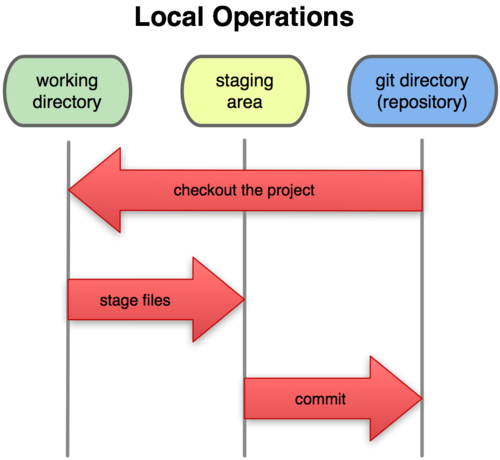
\includegraphics{18333fig0106-tn}
  \caption{Working directory, staging area e git directory. Immagine presa da:
    \url{http://progit.org/book/ch1-3.html}.}
\end{figure}
Prima di iniziare a metterci al lavoro c'è un'ultima cosa da sapere su Git.  I
file possono trovarsi in tre stati chiamati, in inglese, \emph{committed},
\emph{modified} e \emph{staged}. \emph{Commited} significa che il file è stato
salvato nel proprio database locale; \emph{modified} indica che il file è stato
modificato ma non ancora salvato nel database con un \emph{commit};
\emph{staged} significa che il file è stato modificato e la sua versione attuale
verrà salvata nel database con il \emph{commit} successivo, cioè è preparato per
essere aggiunto nella nuova revisione. Un progetto Git può quindi essere
suddiviso in tre sezioni principali: la \emph{git directory}, la
\emph{working directory} e la \emph{staging area}. La prima è dove Git conserva
i metadati e gli oggetti del database del proprio progetto. La
\emph{working directory} è, come dice il nome stesso, la ``cartella di lavoro'',
ossia una copia di una versione del progetto a nostra disposizione per l'uso e
la modifica dei file. L'ultima sezione, la \emph{staging area}, è un semplice
file, generalmente contenuto nella cartella Git, che conserva le informazioni su
ciò che dovrà entrare nel \emph{commit} successivo.

Con Git si lavora più o meno così:
\label{list:lavoro-git}
\begin{enumerate}
\item si modifica uno o più file presenti nella \emph{working directory};
\item si aggiunge un suo \emph{snapshot}, cioè una loro copia, nella
  \emph{staging area};
\item si esegue un \emph{commit}, cioè l'operazione con la quale i file vengono
  copiati così come sono presenti alla \emph{staging area} all'interno della Git
  \emph{directory} in maniera definitiva. Al \emph{commit} viene associato
  l'\emph{hash} che identifica univocamente la versione del progetto così
  salvata.
\end{enumerate}
Se una particolare versione di un file si trova nella cartella git è considerato
\emph{committed}. Se è stato modificato e aggiunto alla \emph{staging area} esso
è detto \emph{staged}. Se è stato modificato da quando è stata aperta la cartella
di lavoro ma non ancora aggiunto alla \emph{staging area} allora il file è detto
\emph{modified}.

\chapter{Git e \LaTeX}
\label{cha:git-latex}

Vogliamo sviluppare un documento con \LaTeX, utilizzando Git come VCS.  Git non
funziona in modo particolarmente esotico. Si tratta semplicemente di creare una
directory, di posizionare in essa i nostri file \filestyle{.tex} e di dire a Git
di considerare tale directory come un \emph{repository}.

\section{Creazione e inizializzazione del \emph{repository}}
\label{sec:iniz-repo}

\begin{lstlisting}
~$ mkdir progetto
~$ cd progetto
~/progetto$ touch np_main.tex
~/progetto$ git init
~/progetto$ git add .
~/progetto$ git commit -am "Inizializzazione del nuovo progetto"
\end{lstlisting}
Vediamo con calma i singoli passaggi.  I primi tre comandi servono
rispettivamente per creare la directory (\texttt{mkdir} \meta{nome directory}),
per spostarsi al suo interno (\texttt{cd} \meta{nome directory}) e per creare un
file vuoto chiamato \filestyle{np\_main.tex} (\texttt{touch} \meta{nome file}).

I passaggi successivi, eseguiti sempre dati dall'interno della cartella in cui
si troverà il progetto, sono quelli specifici di Git:
\begin{itemize}
\item con \texttt{git init} si crea un nuovo \emph{repository} vuoto, cioè
  essenzialmente la cartella nascosta chiamata \filestyle{.git/} che conterrà
  l'intero database.  Questo comando va dato solo al momento della creazione di
  un nuovo \emph{repository} e poi non sarà più necessario riutilizzarlo;
\item \texttt{git add .} aggiunge l'argomento (in questo caso `\filestyle{.}',
  che è un'abbreviazione del percorso della cartella in cui siamo posizionati)
  alla \emph{staging area} del \emph{repository} appena creato;
\item col comando \texttt{commit -am "nota di versione"} effettuiamo il commit
  che, come detto, salva una copia dei file contenuti nella \emph{staging area}
  all'interno del database.  Nella cronologia delle modifiche, a questa
  operazione risulterà associato il messaggio \texttt{"nota di versione"}.
\end{itemize}
Così facendo saremo già pronti a lavorare con il nostro editor di fiducia sul
file \filestyle{.tex} appena creato.

Per continuare il lavoro sul nostro documento e registrare i suoi cambiamenti
dobbiamo eseguire le seguenti operazioni (il seguente elenco puntato deve essere
confrontato con quello presente nel paragrafo~\ref{sec:git} a
pagina~\pageref{list:lavoro-git}):
\begin{enumerate}
\item si modificano i file del codice sorgente presenti nella con il nostro
  editor di testo di fiducia, oppure se ne aggiungono di nuovi (per esempio
  possono essere aggiunte nuove figure);
\item si aggiungono i file che vogliamo registrare nel successivo \emph{commit}
  alla \emph{staging area} con il comando \texttt{git add} \meta{file}, dove al
  posto di \meta{file} va sostituito l'elenco, separato da uno spazio, dei file
  di interesse. Per maggiori informazioni sull'aggiunta di file a un progetto
  Git vedi il paragrafo~\ref{sec:aggiungere-rimuovere-file};
\item si effettua un \emph{commit} con il comando \texttt{git commit}.  A questo
  punto si aprirà l'editor di testo predefinito di Git per l'inserimento del
  messaggio del \emph{commit}.  Vedi il
  paragrafo~\ref{sec:configurazioni-basilari} per sapere come configurare
  l'editor predefinito di Git e il paragrafo~\ref{sec:messaggi-commit} per
  maggiori informazioni sui messaggi dei \emph{commit}.
\end{enumerate}
I punti 2 e 3 possono essere eseguiti insieme se si vogliono aggiungere alla
\emph{staging area} tutti i file che risultano \emph{modified} nella
\emph{working directory} utilizzando il comando \texttt{git commit -a}.

Prima di eseguire un \emph{commit} si possono modificare più file, se ne possono
aggiungere di nuovi o se ne possono cancellare altri. Nel \emph{commit} verranno
memorizzati tutti i cambiamenti presenti nella \emph{staging area} e solamente
quelli, cioè non verranno considerati i file modificati ma non preparati per la
nuova revisione.

\subsection{Messaggi dei \emph{commit}}
\label{sec:messaggi-commit}

In Git, a differenza di altri software VCS, è necessario specificare un
messaggio di \emph{commit} non vuoto.  Se quando registriamo un nuovo
\emph{commit} con il comando \texttt{git commit} non specifichiamo un messaggio
con l'opzione \texttt{-m} si aprirà l'editor di testo associato di default a Git
in cui potremo scrivere il messaggio del \emph{commit}.  Se si utilizza un
editor di testo per scrivere il messaggio di un \emph{commit} è possibile
inserire messaggi estesi su più righe.  Generalmente si utilizza la seguente
convenzione:
\begin{itemize}
\item nella prima riga del messaggio, che non deve superare i 50 caratteri, si
  inserisce una breve e riassuntiva descrizione del \emph{commit} che si sta
  registrando. Il testo del messaggio in questo primo rigo può non essere
  correttamente formattato, per esempio può essere assente la punteggiatura o un
  corretto utilizzo dei caratteri maiuscoli;
\item si lascia la seconda riga vuota e a partire dalla terza si scrive un
  paragrafo contenente una descrizione più dettagliata delle modifiche
  apportate. Il testo di questo paragrafo deve utilizzare la punteggiatura
  opportuna e i caratteri maiuscoli dove necessario. Anche le righe di questo
  paragrafo non dovrebbero superare i 72 caratteri;
\item si possono inserire altri paragrafi per descrivere ulteriormente le
  modifiche lasciando una riga vuota fra un paragrafo e il successivo e seguendo
  le convenzioni illustrate nel punto precedente.
\end{itemize}

Nei messaggi il carattere \lstinline|#| viene interpretato come carattere di
commento e ha lo stesso utilizzo del carattere \lstinline[language=TeX]|%| in
\LaTeX, cioè tutto ciò che in una riga si trova alla destra del carattere
\lstinline|#| verrà ignorato. Si noti che all'apertura dell'editor di testo per
la modifica del messaggio sono presenti, alla fine del file, delle righe di
commento contenenti delle informazioni relative al \emph{commit} che si sta
registrando. Queste righe possono essere ignorate.

\section{Aggiungere e rimuovere file del progetto}
\label{sec:aggiungere-rimuovere-file}

Per controllare lo stato di un \emph{repository} Git esiste il comando
\texttt{git status}.  Questo comando ci permette di monitorare costantemente la
situazione di tutti i file e fornisce spesso dei suggerimenti utili (in lingua
inglese) sulle operazioni che possono essere eseguite sui file.  Se dopo aver
effettuato un \emph{commit} si sono modificati dei file, l'output di questo
comando sarà qualcosa di simile a ciò che segue
\begin{lstlisting}
# On branch master
# Changes not staged for commit:
#   (use "git add <file>..." to update what will be committed)
#   (use "git checkout -- <file>..." to discard changes in working directory)
#
#	modified:   TODO
#	modified:   git4latex.tex
#
no changes added to commit (use "git add" and/or "git commit -a")
\end{lstlisting}
In questo esempio nella \emph{working directory} sono presenti due file, tutti e
due \emph{modified} ma non \emph{staged}, come ben spiegato da Git. Nell'ultima
riga dell'output Git ci suggerisce anche come aggiungere i file alla
\emph{staging area}, cioè usando i già visti \texttt{git add} \meta{file} oppure
\texttt{git commit -a}.  Se aggiungiamo il file \filestyle{git4latex.tex} alla
\emph{staging area} l'output di \texttt{git status} diventerà
\begin{lstlisting}
$ git add git4latex.tex
$ git status
# On branch master
# Changes to be committed:
#   (use "git reset HEAD <file>..." to unstage)
#
#	modified:   git4latex.tex
#
# Changes not staged for commit:
#   (use "git add <file>..." to update what will be committed)
#   (use "git checkout -- <file>..." to discard changes in working directory)
#
#	modified:   TODO
#
\end{lstlisting}
Adesso \texttt{git4latex.tex} compare nell'elenco dei file che faranno parte del
prossimo \emph{commit}.  Ci viene anche suggerito come rimuovere un file dalla
\emph{staging area}, usando \texttt{git reset HEAD} \meta{file}, ma riprenderemo
questo discorso nel paragrafo~\ref{sec:annullare-modifiche-non-salvate}.  Non è
necessario che tutti i file siano spostati nella \emph{staging area} prima di
effettuare un nuovo \emph{commit}, possiamo spostare solo quelli che vogliamo
registrare nella revisione successiva.

Se dopo aver spostato un file nella \emph{staging area} lo modifichiamo
nuovamente, questo apparirà sia nell'elenco dei file che faranno parte del nuovo
\emph{commit} sia in quello dei file \emph{modified} ma non \emph{staged}
\begin{lstlisting}
# On branch master
# Changes to be committed:
#   (use "git reset HEAD <file>..." to unstage)
#
#	modified:   git4latex.tex
#
# Changes not staged for commit:
#   (use "git add <file>..." to update what will be committed)
#   (use "git checkout -- <file>..." to discard changes in working directory)
#
#	modified:   TODO
#	modified:   git4latex.tex
#
\end{lstlisting}
Succede questo perché Git non ricorda semplicemente l'elenco dei file che sono
pronti per entrare nella nuova revisione, ma memorizza nella \emph{staging area}
una copia del file così com'era al momento dell'esecuzione del comando
\texttt{git add} \meta{file}.  Prima di effettuare il \emph{commit} quindi è
bene controllare che il file sia solo fra quelli \emph{to be committed} e non
anche fra i file \emph{not staged for commit}, per evitare di inserire nel
\emph{commit} un file alla versione sbagliata.  Un metodo semplice per rimediare
a questo pericolo è quello di usare \texttt{git commit -a}, ma questo è
possibile solo se si vogliono aggiungere al \emph{commit} tutti i file che
risultano \emph{modified}.

Il comando \texttt{git add} permette di aggiungere al \emph{repository}
qualsiasi file presente nella \emph{working directory}, anche quelli non ancora
conosciuti da Git.\footnote{In effetti subito dopo aver creato il
  \emph{repository} con \texttt{git init}, Git non conosceva nessun file, noi
  glieli abbiamo presentati con \texttt{git add} \meta{file}.}  Per esempio, se
abbiamo creato un file per la bibliografia, chiamato
\filestyle{bibliografia.bib}, del nostro documento la situazione sarà la
seguente
\begin{lstlisting}
$ git status
# On branch master
# Untracked files:
#   (use "git add <file>..." to include in what will be committed)
#
#	bibliografia.bib
nothing added to commit but untracked files present (use "git add" to track)
\end{lstlisting} %$
I file \emph{untracked} sono quelli non ancora seguiti da Git poiché non ancora
conosciuti. Come avrete probabilmente già capito, e come suggerito anche
dall'output del comando, per rendere noto a Git il file dovremo usare
\texttt{git add bibliografia.bib}.  Se avessimo provato a effettuare
direttamente un \emph{commit} con \texttt{git commit -a} avremmo ottenuto la
seguente risposta
\begin{lstlisting}
$ git commit -am "aggiungo bibliografia"
# On branch master
# Untracked files:
#   (use "git add <file>..." to include in what will be committed)
#
#       bibliografia.bib
nothing added to commit but untracked files present (use "git add" to track)
\end{lstlisting} %$
Git si sarebbe accorto della presenza del nuovo file, ma non lo avrebbe aggiunto
automaticamente al progetto. D'altra parte, se avesse rilevato delle modifiche
ai file precedentemente aggiunti al progetto, non si sarebbe nemmeno curato di
comunicarci che il nuovo file non è ancora stato aggiunto al progetto. Si
sarebbe infatti limitato a salvare le modifiche ai file che gli abbiamo
precedentemente detto di gestire. Solo con il comando \texttt{git status}
possiamo controllare con certezza lo stato di tutti i file del
\emph{repository}.

Oltre ad aggiungere file a un \emph{repository} è possibile, naturalmente, anche
rimuoverli.  La sintassi è la seguente: \texttt{git rm} \meta{file}, in cui a
\meta{file} va sostituito, come al solito, l'elenco dei file che si vogliono
cancellare.  Questo comando elimina il file dalla \emph{working directory} e
aggiunge la cancellazione del file alla \emph{staging area}, ma non crea un
nuovo \emph{commit} che dovrà quindi essere eseguito esplicitamente, senza però
aver bisogno di fare altro.  Poiché la cancellazione è memorizzata nella
\emph{staging area}, per rimuovere l'eliminazione accidentale di un file, prima
di effettuare un \emph{commit}, eseguita con \texttt{git rm} \meta{file},
possiamo usare \texttt{git reset HEAD} \meta{file}.  Adesso la modifica è
presente solo nella \emph{working directory} (cioè il file è assente dalla
cartella di lavoro), per ripristinarlo useremo \texttt{git checkout -{}-}
\meta{file}.  Non c'è bisogno di ricordare a memoria tutte le operazioni per il
ripristino del file,\footnote{Queste operazioni dovrebbero risultare più chiare
  dopo avere letto il paragrafo~\ref{sec:annullare-modifiche-non-salvate}.}
queste infatti sono suggerite dall'output di \texttt{git status}.
\begin{lstlisting}
$ git rm bibliografia.bib
rm 'bibliografia.bib'
$ git status
# On branch master
# Changes to be committed:
#   (use "git reset HEAD <file>..." to unstage)
#
#	deleted:    bibliografia.bib
#
$ git reset HEAD bibliografia.bib
Unstaged changes after reset:
M	bibliografia.bib
$ git status
# On branch master
# Changes not staged for commit:
#   (use "git add/rm <file>..." to update what will be committed)
#   (use "git checkout -- <file>..." to discard changes in working directory)
#
#	deleted:    bibliografia.bib
#
no changes added to commit (use "git add" and/or "git commit -a")
$ git checkout -- bibliografia.bib
$ git status
# On branch master
nothing to commit (working directory clean)
\end{lstlisting}

\subsection{Ignorare file del progetto:
  \texorpdfstring{\filestyle{.gitignore}}{.gitignore}}
\label{sec:ignorare-file}
% TODO: rivedere questa sezione

Come ormai sappiamo bene, per aggiungere dei file alla \emph{staging area}
dobbiamo usare il comando \texttt{git add} \meta{file}, in cui a \meta{file}
andrà sostituito l'elenco dei file, separati da uno spazio, che si vogliono
includere nel \emph{commit} successivo. Si può scegliere di procedere in due
modi: aggiungere indiscriminatamente tutti i file della cartella corrente al
progetto che stiamo sviluppando; oppure aggiungere un singolo file. Nel primo
caso dovremmo ripetere il comando già usato in fase di inizializzazione:
\begin{lstlisting}
$ git add .
\end{lstlisting}
Nel secondo caso aggiungiamo un singolo file:
\begin{lstlisting}
$ git add np_secondary.tex
\end{lstlisting}
Per quanto possa sembrare eccessivo, io preferisco usare il secondo comando.  Mi
accade con estrema frequenza di dover aggiungere dei file a un progetto, e
spesso sono fin troppo distratto da quel che sto scrivendo per occuparmi di quel
che Git si aspetta da me.  L'aggiunta indiscriminata di ogni file nella
directory al \emph{repository} presenta però delle controindicazioni.  La più
ovvia per chi lavora con \LaTeX{} è la seguente: nel corso dell'elaborazione di
un testo inevitabilmente si procederà alla generazione del documento in pdf a
partire dai sorgenti; \LaTeX{} provvederà quindi alla generazioni di una serie
di file ausiliari (\filestyle{.toc}, \filestyle{.out}, \dots), nonché di un
\textsc{pdf} più o meno inutile. Se eseguissimo il comando \texttt{git add .}
subito dopo una compilazione, evidentemente Git aggiungerebbe alla \emph{staging
  area} anche i vari file di lavoro, dal pdf, ai file di log.  Per ovviare a
questo inconveniente, e continuare pigramente a eseguire \texttt{git add .}, è
utile creare nella nostra directory di un file denominato
\filestyle{.gitignore}.
\begin{lstlisting}
$ echo "*.log" >> .gitignore
$ echo "*.pdf" >> .gitignore
$ echo "*.blg" >> .gitignore
$ echo "*.bbl" >> .gitignore
$ echo "*.aux" >> .gitignore
$ echo "*-blx.bib" >> .gitignore
$ echo "*.out" >> .gitignore
$ echo "*~" >> .gitignore
$ git add .gitignore
$ git commit -am "Aggiunto il file .gitignore"
\end{lstlisting}

Mediante questo file, istruiamo Git a proposito di tutti i file che non fanno
effettivamente parte del progetto, pur essendo presenti nella cartella.  Da
questo momento in poi Git si limiterà a ignorarli, il che ci permette di
eseguire prudenzialmente il comando \texttt{git add .} prima di ogni
\emph{commit}. Generalmente Git è usato per gestire solo il codice sorgente di
un progetto, sia esso un programma o un documento \LaTeX, quindi è buona norma
aggiungere all'elenco dei file ignorati tutti quei file, ausiliari o di output,
che vengono generati nella fase di compilazione, del programma o documento, ma
che non fanno parte del codice sorgente propriamente detto. Nel caso di un
documento \LaTeX{} saranno i file con estensione, per esempio, \filestyle{.log},
\filestyle{.aux}, \filestyle{.toc} (per i file ausiliari temporanei) e
\filestyle{.pdf} (per il file di output).  L'aggiunta del \textsc{pdf} finale
comporterebbe un inutile duplicato nella cronologia dato che è già presente
l'intero codice sorgente e inoltre appesantisce notevolmente l'intero
\emph{repository}.  Se si vuole distribuire il \textsc{pdf} è preferibile
caricarlo su un apposito sito di \emph{file hosting}.\footnote{Alcuni siti, come
  \url{https://bitbucket.org} e \url{http://sourceforge.net}, che offrono la
  possibilità di ospitare \emph{repository} git remoti permettono inoltre di
  caricare dei file esterni al \emph{repository} proprio come un classico sito
  di \emph{file hosting}.}

\section{Consultare la cronologia}
\label{sec:consultare-cronologia}

In Git è possibile, naturalmente, consultare la cronologia dei \emph{commit}
registrati nel \emph{repository} in uso.  Il comando da usare è \texttt{git
  log}.  L'output di questo comando, senza ulteriori opzioni, sarà qualcosa di
questo tipo
\begin{lstlisting}
commit 9e1691276ba70443c56c214a52088814a5f25ec5
Author: Pietro Giuffrida <pietro.giuffri@gmail.com>
Date:   Sat Oct 2 19:32:12 2010 +0200

    un po' di pulizia

commit 86ee0a0525dd759bb49308b58cf3e761471a04cd
Author: Pietro Giuffrida <pietro.giuffri@gmail.com>
Date:   Sat Oct 2 19:31:24 2010 +0200

    prime due sezioni

commit 43c5858e91a7090b834dd9f09ddfae1061901ee4
Author: Pietro Giuffrida <pietro.giuffri@gmail.com>
Date:   Sat Oct 2 18:53:30 2010 +0200

    Ho solo iniziato a lavorare
\end{lstlisting}
È possibile muoversi nella cronologia con i tasti freccia. Nella prima riga di
ogni revisione (che inizia con \texttt{commit}) è riportato l'\emph{hash} esteso
corrispondente, nella seconda l'autore (\texttt{Author}) del \emph{commit},
quindi la data di salvataggio (\texttt{Date}) e il messaggio descrittivo.

È possibile mostrare solo l'elenco degli ultimi $n$ \emph{commit} aggiungendo
l'opzione \texttt{-}\meta{n}. Dunque per mostrare solo l'ultimo \emph{commit}
possiamo usare il comando \texttt{git commit -1}.  Si può consultare la
cronologia relativa a uno o più specifici file e non all'intero
\emph{repository} passando come argomento del comando l'elenco dei file di
interesse, separati da uno spazio: \texttt{git log -{}-} \meta{file}.  Se si
vuole visualizzare solo l'elenco degli ultimi \texttt{n} \emph{commit} relativi
a un determinato elenco di file si possono utilizzare contemporaneamente
l'opzione \texttt{-}\meta{n} e l'argomento \meta{file}.  Per esempio il comando
\texttt{git log -3 -{}- main.tex capitolo2.tex} mostrerà gli ultimi tre
\emph{commit} che hanno modificato i file \filestyle{main.tex} e
\filestyle{capitolo2.tex}.  Il doppio trattino \texttt{-{}-} serve per far
capire a Git che tutto ciò che segue è l'elenco dei file.  In generale non è
obbligatorio utilizzarlo ma diventa necessario per evitare ambiguità nel caso in
cui ci siano rami o etichette con lo stesso nome del file.

Come abbiamo visto, in maniera predefinita \texttt{git log} mostra solo alcune
informazioni dei \emph{commit}. Per mostrare anche le modifiche apportate in
ciascun \emph{commit} nel formato \texttt{diff} si può utilizzare l'opzione
\texttt{-p}.  Per esempio, l'esecuzione del comando \texttt{git log -1 -p} potrà
dare un output di questo tipo:
\begin{lstlisting}
commit 5a5f793b0780d2c3352239beca3fc8de432a71b9
Author: Paolino Paperino <paolino.paperino@example.org>
Date:   Fri Oct 8 22:32:51 2010 +0200

    rimuovo pacchetto `xcolor'

    Ora che l'ambiente `lstlisting' non e' piu' colorato
    non e' piu' necessario.

diff --git a/git4latex.tex b/git4latex.tex
index 74a1474..a84fb27 100644
--- a/git4latex.tex
+++ b/git4latex.tex
@@ -26,9 +26,6 @@
 \usepackage[font=small,format=hang]{caption}
 \usepackage{graphicx}

-\usepackage[dvipsnames, usenames]{xcolor}
-\definecolor{GY}{named}{GreenYellow} % SkyBlue
-
 \usepackage{listings}
 \usepackage{fourier}
\end{lstlisting}

Segnaliamo infine un'altra utile opzione che serve per mostrare come
informazioni del \emph{commit} solo l'\emph{hash} in formato breve e la prima
riga del messaggio.  Questa opzione si chiama \texttt{-{}-oneline} ed è utile se
si vuole trovare rapidamente l'\emph{hash} di un \emph{commit} sfogliando le
prime righe dei messaggi di tutti i commit.  Per esempio, il primo output di
\texttt{git log} riportato all'inizio di questo paragrafo, con l'opzione
\texttt{-{}-oneline} apparirebbe così:
\begin{lstlisting}
$ git log --oneline
9e16912 un po' di pulizia
86ee0a0 prime due sezioni
43c5858 Ho solo iniziato a lavorare
\end{lstlisting} %$

Per maggiori informazioni è possibile consultare la documentazione di
\texttt{git log} con il comando \texttt{man git-log}.

\section{Annullare e cambiare modifiche precedenti}
\label{sec:annullare-modifiche}

Ci sono vari modi per cambiare le modifiche effettuate in un \emph{repository}
Git, ma per scegliere quella adatta bisogna sapere che tipo di modifica si
desidera annullare. In questo paragrafo presenteremo alcune delle situazioni più
frequenti che si possono incontrare.

\subsection{Annullare modifiche non ancora salvate}
\label{sec:annullare-modifiche-non-salvate}

Se si vogliono annullare tutte le modifiche effettuate a dei file ma non ancora
registrate in un \emph{commit} si può usare il comando
\begin{lstlisting}
$ git reset --hard HEAD
\end{lstlisting} %$
In questo modo l'intera \emph{working directory} viene ripristinata alla stato
corrispondente all'ultimo \emph{commit} della cronologia, indicato con
\texttt{HEAD}.

Se si vogliono riportare allo stato dell'ultimo \emph{commit} registrato solo
determinati file che sono \emph{modified} ma non ancora \emph{staged}, adottando
la terminologia vista all'inizio, senza toccare la restante
\emph{working directory} si può utilizzare il comando
\begin{lstlisting}
$ git checkout -- £\meta{file}£
\end{lstlisting} %$
in cui a \meta{file} va sostituito l'elenco dei file, separati da uno spazio,
che si vogliono ripristinare. Le opzioni e gli argomenti che il comando
\texttt{git commit} può accettare sono numerosi e le operazioni che verranno
eseguite possono essere diverse a seconda delle istruzioni fornite (ma non è
scopo della presente guida spiegare nei dettagli il completo funzionamento di
Git), il doppio trattino \texttt{-{}-} serve per far capire a Git, senza
possibilità di ambiguità, che tutto ciò che si trova dopo è l'elenco dei file e
l'operazione da eseguire è quella qui descritta. Il doppio trattino può essere
omesso se non ci sono possibili ambiguità, per esempio se il file da passare
come argomento non ha lo stesso nome di uno dei \emph{branch} (vedi
paragrafo~\ref{sec:branch}) del \emph{repository}. Il comando \texttt{git
  checkout -{}-} \meta{file} può anche essere usato per ripristinare file
accidentalmente cancellati prima effettuare un nuovo \emph{commit}. In questo
caso l'uso del doppio trattino è necessario dal momento che il file cancellato
non si trova nella \emph{working directory} e Git non capirebbe che \meta{file}
è con certezza un elenco di file cancellati. Altri modi per ripristinare file
cancellati saranno visti nel paragrafo~\ref{sec:ripristinare-file}.

Se invece si vogliono solo togliere uno o più file dalla \emph{staging area} ma
lasciare intatta la \emph{working directory} si può usare il comando
\begin{lstlisting}
$ git reset HEAD £\meta{file}£
\end{lstlisting} %$
Come al solito, a \meta{file} va sostituito l'elenco dei file di interesse,
separati da uno spazio.  I file tolti dalla \emph{staging area} possono poi
anche essere ripristinati allo stato del \emph{commit} precedente usando il
comando \texttt{git checkout -{}-} \meta{file} illustrato qui sopra.

\subsection{Modificare l'ultimo \emph{commit} non inviato in remoto}
\label{sec:modifica-ultimo-commit-non-remoto}

L'opzione \texttt{-{}-amend} del comando \texttt{git commit} permette di
modificare l'ultimo \emph{commit}.  Se dopo aver salvato un \emph{commit} ci
accorgiamo che dobbiamo correggerlo (per esempio perché ci siamo dimenticati
apportare una modifica o di aggiungere un file), possiamo normalmente modificare
i file di interesse, aggiungerli alla \emph{staging area} con il comando
\texttt{git add} \meta{file}\footnote{Se ci si era dimenticati di aggiungere un
  file nuovo o modificato alla \emph{staging area} prima di effettuare il
  \emph{commit} precedente, sarà sufficiente eseguire \texttt{git add}
  \meta{file} senza dover modificare ulteriormente alcun file.}  e poi, invece
di effettuare un nuovo \emph{commit} con \texttt{git commit}, eseguire il
comando \texttt{git commit -{}-amend} che modificherà l'ultimo \emph{commit}
della cronologia.  A questo punto si aprirà la solita interfaccia che compare al
momento del salvataggio di un \emph{commit}: è possibile modificare il
messaggio, altrimenti è sufficiente uscire direttamente dall'interfaccia.

Se bene sia in realtà possibile, è altamente sconsigliato modificare un
\emph{commit} già inviato in remoto con \texttt{git push} (vedi il
paragrafo~\ref{sec:repository-on-line}) se il \emph{repository} è condiviso con
altre persone, poiché i loro \emph{repository} non potranno più continuare a
essere sincronizzati con il \emph{repository} centrale.  Quindi, se si condivide
il progetto con altri utenti è preferibile riscrivere la cronologia con
\texttt{git commit -{}-amend} solo per \emph{commit} non ancora inviati in
remoto.

\subsection{Annullare un \emph{commit}}
\label{sec:annullare-commit}

Per annullare le modifiche apportate con uno specifico \emph{commit}, creando un
nuovo \emph{commit} si può usare il comando
\begin{lstlisting}
$ git revert £\meta{hash commit}£
\end{lstlisting} %$
in cui a \meta{hash commit} va sostituito l'\emph{hash} del \emph{commit} che si
vuole annullare (vedi il paragrafo~\ref{sec:consultare-cronologia} per sapere
come recuperare l'\emph{hash} abbreviato sfogliando la cronologia delle
modifiche).  Se per esempio la forma abbreviata dell'\emph{hash} corrispondente
al \emph{commit} che si vuole annullare è \texttt{d4fcdbd} il comando da usare è
\begin{lstlisting}
$ git revert d4fcdbd
\end{lstlisting} %$
Dopo aver eseguito il comando si aprirà l'interfaccia per la modifica del
messaggio del nuovo \emph{commit}. Se il \emph{commit} da annullare è l'ultimo
al posto dell'\emph{hash} si può usare il riferimento \texttt{HEAD}: \texttt{git
  revert HEAD}.
% Nella guida non ne parlo perché non so neanche io bene come funzioni, comunque
% segnalo a chi legge questo commento che dovrebbe essere possibile modificare
% vecchi commit non inviati in remoto con `git rebase'. Si veda
% http://book.git-scm.com/4_undoing_in_git_-_reset,_checkout_and_revert.html

\section{Ripristinare file}
\label{sec:ripristinare-file}

In questo paragrafo vedremo come ripristinare file cancellati dal progetto
oppure riportare file ancora presenti nel \emph{repository} a una versione
precedente.

Ipotizziamo a titolo esemplificativo il seguente scenario: abbiamo creato un
file, \filestyle{np\_secondary.tex}, l'abbiamo aggiunto al \emph{repository} Git
con il comando \texttt{git add np\_secondary.tex} e abbiamo eseguito il commit.
Dopo di ciò abbiamo accidentalmente cancellato il file con il comando \texttt{rm
  np\_secondary.tex} e abbiamo effettuato un altro \emph{commit} che ha
registrato la cancellazione del file:
\begin{lstlisting}
$ echo "pippo" >> np_secondary.tex
$ git add np_secondary.tex
$ git commit -am "Ho solo iniziato a lavorare"
$ rm np_secondary.tex
$ git commit -am "Ma ho gia' perso tutto"
\end{lstlisting} %$
Ora chiediamo conto a Git della sua capacità di ripristinare una versione
precedentemente salvata. La prima cosa da fare è consultare la cronologia dei
\emph{commit} precedentemente effettuati, per ottenere l'\emph{hash} della
versione che vogliamo ripristinare. Il comando appropriato quindi, per quanto
visto nel paragrafo~\ref{sec:consultare-cronologia}, è \texttt{git log -{}-}
\meta{file}.  Poiché è sufficiente conoscere l'\emph{hash} in forma abbreviata
dell'ultima revisione in cui il file era ancora presente nel progetto usiamo le
opzioni \texttt{-{}-oneline} e \texttt{-2} (l'ultima revisione in cui comparirà il
file \filestyle{np\_secondary.tex} è quella in cui è stato cancellato, ma a noi
interessa quella precedente)
\begin{lstlisting}
$ git log -2 --oneline -- np_secondary.tex
3802287 Ma ho gia' perso tutto
c21d825 Ho solo iniziato a lavorare
\end{lstlisting} %$
Per ripristinare il file cancellato all'ultima versione in cui ancora era
presente nel progetto possiamo usare il comando \texttt{git checkout} \meta{hash
  del commit} \texttt{-{}-} \meta{file} in cui ad \meta{hash del commit} dovremo
sostituire l'\emph{hash} (eventualmente in forma abbreviata) del \emph{commit} a
cui vogliamo ripristinare i file elencati in \meta{file}.  Quindi nel nostro
esempio per ripristinare il file \filestyle{np\_secondary.tex} alla versione
presente nel \emph{commit} \texttt{c21d825} useremo il comando
\begin{lstlisting}
$ git checkout c21d825 -- np_secondary.tex
\end{lstlisting} %$

Il comando \texttt{git checkout} \meta{hash del commit} \texttt{-{}-}
\meta{file} permette di riportare qualsiasi file elencato in \meta{file} alla
versione \meta{hash del commit}, anche se non cancellato e ancora presente nel
progetto, sempre utilizzando la stessa sintassi.  Chiaramente, Git permette il
ripristino esclusivamente dei file aggiunti al \emph{repository} ed
esclusivamente di versioni esplicitamente salvate mediante il comando
\texttt{git commit}.  I salvataggi effettuati tra un \emph{commit} e l'altro non
sono quindi ricostruibili.

L'uso di \texttt{git checkout -{}-} \meta{file} visto nel
paragrafo~\ref{sec:annullare-modifiche-non-salvate} è un caso particolare di
quello qui spiegato, in cui si ripristina un file alla versione presente
nell'ultimo \emph{commit}, nel caso in cui non ne viene indicato esplicitamente
uno differente.

È inoltre possibile visionare nel terminale una precedente versione di un file
con la sintassi
\begin{lstlisting}
$ git show £\meta{hash del commit} \meta{file}£ 
\end{lstlisting}

\section{Gestione dei \emph{branch}}
\label{sec:branch}

Con il comando \texttt{git status} possiamo controllare lo stato del progetto,
per esempio se ci sono dei file che sono stati modificati ma non ancora salvati
nel \emph{commit} e così via. Un tipico output di questo comando è:
\begin{lstlisting}
$ git status
# On branch master
nothing to commit (working directory clean)
\end{lstlisting} %$
L'ultima riga del messaggio significa che non sono presenti file modificati (a
parte eventualmente quelli ignorati con il file \filestyle{.gitignore}) dopo
l'ultimo \emph{commit}.  Ma cosa significa \texttt{On branch master}?
\emph{Branch} in inglese significa ``ramo'' e Git ci dà la possibilità di creare
una linea di sviluppo per il nostro progetto parallela a quella iniziale
(chiamata \emph{master} in Git) ma con delle modifiche che divergono da questa
proprio come il ramo di un albero diverge dal tronco centrale (e per completare
questa analogia botanica la linea di sviluppo centrale è a volte chiamata
proprio \emph{trunk}, cioè ``tronco'').

\subsection{Perché creare un \emph{branch}?}
\label{sec:perche-branch}

Le risposte a questa domanda possono essere diverse. Una potrebbe essere, per
esempio perché abbiamo intenzione di scrivere un capitolo per il nostro documento
\LaTeX{} ma non siamo sicuri che sia veramente necessario: possiamo allora creare
un \emph{branch} nel quale scriveremo solo questo capitolo mentre nel ramo
principale \emph{master} continueremo normalmente a modificare il documento.
Quando il capitolo sarà pronto, se il risultato sarà soddisfacente potremo
procedere alla funsione del ramo ``sperimentale'' in quello principale, operazione
chiamata \emph{merge} in gergo, e nel nostro documento ``comparirà magicamente''
il capitolo che abbiamo sviluppato nel \emph{branch}, in caso contrario possiamo
semplicemente cancellare il \emph{branch}, come se avessimo potato il ramo
indesiderato dell'albero.

Un altro caso in cui può essere utile creare un \emph{branch} è quello in cui si
lavori a più mani su un documento: mentre voi scrivete il vostro documento un
vostro amico vi chiede di collaborarvi e anch'egli userà Git per tenere traccia
delle sue modifiche.  Lui creerà un suo ramo di sviluppo in modo che voi potrete
continuare a redigere il vostro documento senza che le sue modifiche vadano a
confliggere con le vostre.  Alla fine il vostro amico vi farà vedere il
risultato delle sue modifiche: se le apprezzate potete effettuare il
\emph{merge} del suo ramo nel vostro, altrimenti potete dirgli che le sue
modifiche non vi piacciono e il suo \emph{branch} sarà cancellato.

\begin{figure}
  \centering
  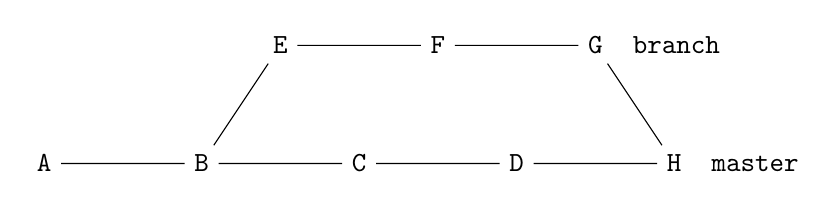
\begin{tikzpicture}
    \node (A) at (0,0) {\texttt{A}};
    \node (B) at (2,0) {\texttt{B}};
    \node (C) at (4,0) {\texttt{C}};
    \node (D) at (6,0) {\texttt{D}};
    \node (H) at (8,0) {\texttt{H}};
    \node (E) at (3,1.5) {\texttt{E}};
    \node (F) at (5,1.5) {\texttt{F}};
    \node (G) at (7,1.5) {\texttt{G}};
    \draw (A) -- (B) -- (C) -- (D) -- (H) node[right=10] {\texttt{master}} --
          (G) node[right=10] {\texttt{branch}} -- (F) -- (E) -- (B);
  \end{tikzpicture}
  \caption{Flusso delle modifiche effettuato nel ramo principale \texttt{master}
    e nel ramo secondario \texttt{branch}.  Il ramo \texttt{branch} viene fuso
    nel ramo \texttt{master} con il \emph{commit} \texttt{H}.}
  \label{fig:schema-branch}
\end{figure}
Nella figura~\ref{fig:schema-branch} è rappresentato un semplice grafico dello
sviluppo di un progetto in cui è stato effettuato un \emph{branching}.  Nel ramo
\texttt{master} abbiamo effettuato le modifiche indicate con \texttt{A} e
\texttt{B}.  A questo punto creiamo il ramo \texttt{branch}.  D'ora in poi le
modifiche effettuate su un ramo avranno valore solo su quello: continuiamo a
lavorare normalmente su \texttt{master} apportando le modifiche indicate con
\texttt{C} e \texttt{D}, mentre in \texttt{branch} avremo effettuato le
modifiche \texttt{E}, \texttt{F} e \texttt{G} che apparterranno solo a questo
ramo.  Decidiamo quindi di fondere i due rami perché le modifiche fatte in
\texttt{branch} ci soddisfano: con la modifica \texttt{H} tutte le modifiche
effettuate in \texttt{branch} verranno importate nel ramo principale e potremo
continuare lì il nostro lavoro.

\subsection{Creare e cancellare un \emph{branch}}
\label{sec:creare-cancellare-branch}

Per creare un \emph{branch} dobbiamo usare il comando \texttt{git branch}
\meta{nome branch}.  Se il comando va a buon fine non ci sarà nessun output,
possiamo però controllare l'elenco dei rami esistenti con il comando \texttt{git
  branch} senza alcun ulteriore argomento:
\begin{lstlisting}
$ git branch foo
$ git branch
  foo
* master
\end{lstlisting}
L'asterisco vicino a \texttt{master} sta a indicare che al momento ci troviamo
nel \emph{branch} \texttt{master}.  Per spostarci in un altro \emph{branch}
usiamo il comando \texttt{git checkout} \meta{nome branch}:
\begin{lstlisting}
$ git checkout foo
Switched to branch 'foo'
$ git branch
* foo
  master
\end{lstlisting}
Che significa che ci siamo spostati in un altro \emph{branch}?  Abbiamo cambiato
cartella?  No, siamo sempre nella stessa cartella (possiamo controllarlo con il
comand \texttt{pwd}), ma è stato Git che ha modificato la nostra cartella di
lavoro, la \emph{working directory}, andando a prendere dal suo database
l'ultimo \emph{snapshot}, l'ultima ``fotografia'', del \emph{branch} che gli
abbiamo richiesto.  In alternativa a \texttt{git branch} \meta{nome branch}, per
creare un nuovo ramo si può usare il comando \texttt{git checkout -b} \meta{nome
  branch} che in più effettua direttamente il \emph{checkout} del nuovo
\emph{branch}:
\begin{lstlisting}
$ git checkout -b foo
Switched to a new branch 'foo'
\end{lstlisting} %$

Un \emph{branch} appena creato e non modificato è uguale al ramo da cui è stato
creato, contiene i suoi stessi file e la stessa cronologia.  Lo sviluppo del
progetto può continuare in maniera identica a quella vista prima (cioè si usano
i soliti comandi \texttt{git add} e \texttt{git commit}), però le modifiche
apportate in questo \emph{branch} non compariranno nel registro di quello
principale.  Possiamo verificarlo controllando i rispettivi log:
\begin{lstlisting}
$ git branch
* foo
  master
$ git log
commit c71da4fe9bf764274e67a2326ec1dc3911691928
Author: Pietro Giuffrida <pietro.giuffri@gmail.com>
Date:   Sat Oct 9 19:09:56 2010 +0200

    primo commit nel branch `foo'

commit e17384278acadbfefefebf0ced4e7103005a597c
Author: Pietro Giuffrida <pietro.giuffri@gmail.com>
Date:   Sat Oct 9 19:08:46 2010 +0200

    iniziamo il nuovo progetto
$ git checkout master
Switched to branch 'master'
$ git log
commit e17384278acadbfefefebf0ced4e7103005a597c
Author: Pietro Giuffrida <pietro.giuffri@gmail.com>
Date:   Sat Oct 9 19:08:46 2010 +0200

    iniziamo il nuovo progetto
\end{lstlisting}

Per cancellare un ramo di cui si è già effettuato il \emph{merge} con il ramo
principale (vedremo più avanti come si fa) si usa l'opzione \texttt{-d} del
comando \texttt{git branch}:
\begin{lstlisting}
$ git branch -d foo
Deleted branch foo (was c71da4f).
\end{lstlisting} %$
Se proviamo a usare l'opzione \texttt{-d} con un ramo di cui non è stato
ancora effettuato il \emph{merge} Git ci avverte:
\begin{lstlisting}
$ git branch -d foo
error: The branch foo' is not fully merged.
If you are sure you want to delete it, run 'git branch -D foo'.
\end{lstlisting} %$
Come al solito Git ci suggerisce i comandi che ci possono tornare utili: se
vogliamo ugualmente cancellare il \emph{branch} che non è stato fuso in quello
principale dobbiamo usare l'opzione \texttt{-D} al posto di \texttt{-d}:
\begin{lstlisting}
$ git branch -D foo
Deleted branch foo (was c71da4f).
\end{lstlisting}

\subsection{Effettuare un \emph{merge}}
\label{sec:merge}

Per effettuare la fusione, \emph{merge}, di due rami si deve utilizzare il
comando \texttt{git merge} \meta{nome branch}, da dare nel ramo in cui si
desidera importare il ramo chiamato \meta{nome branch}.  Se tutto va bene
otterremo un output simile al seguente (supponiamo, per esempio, che il ramo da
importare si chiami \texttt{foo}):
\begin{lstlisting}
$ git merge foo
Updating da45d11..729129c
Fast-forward
 capitolo5.tex |   18 ++++++++++++++++++
 1 files changed, 18 insertions(+), 0 deletions(-)
 create mode 100644 capitolo5.tex
\end{lstlisting} %$
Dopo di ciò possiamo normalmente fare il \emph{commit} con
\texttt{git add .} e \texttt{git commit -am "messaggio di commit"}.

Può verificarsi un problema se uno o più file sono stati modificati nello stesso
punto in tutti e due i rami che si vogliono fondere, dopo che è stato creato il
\emph{branch}. Git, infatti, non è in grado di gestire automaticamente questa
situazione (è uno strumento potente ma non può certo leggere nel nostro pensiero,
non può sapere perché il file è stato modificato diversamente nei due rami) e ci
avverte con un messaggio di questo tipo:
\begin{lstlisting}[language={}]
$ git merge foo
Auto-merging main.tex
CONFLICT (content): Merge conflict in main.tex
Automatic merge failed; fix conflicts and then commit the result.
\end{lstlisting}
Nel presente esempio il file in cui si sono verificati i conflitti si chiama
\filestyle{main.tex}.  Aprendo con il nostro editor di testo troveremo nel punto
in cui si è verificato il conflitto qualcosa di questo tipo:
\begin{lstlisting}[language={},emph={HEAD,foo}]
<<<<<<< HEAD
\usepackage{hyperref}
=======
\usepackage[bookmarks=false,colorlinks=true]{hyperref}
>>>>>>> foo
\end{lstlisting} %$
La zona compresa fra \lstinline|<<<<<<< HEAD| e \lstinline|=======| indica il
contenuto del file presente nel ramo corrente, mentre ciò che è scritto fra
\lstinline|=======| e \lstinline|>>>>>>> foo| è ciò che si trova nel
corrispondente punto dello stesso file \filestyle{main.tex} ma nel ramo
\texttt{foo} che stiamo provando a fondere in \texttt{master}.  Dopo aver
corretto il file come desideriamo che risulti, possiamo finalmente salvarlo ed
effettuare come al solito il \emph{commit}.

\subsection{Copiare un singolo \emph{commit} da un \emph{branch} a un altro}
\label{sec:copiare-un-commit}

Mentre sviluppiamo un \emph{branch} potremmo accorgerci che il \emph{commit}
appena effettuato apporta delle modifiche che possono essere utili anche in un
altro \emph{branch} (come per esempio la correzione di un errore di ortografia o
una modifica al preambolo del documento). Non è necessario effettuare il
\emph{merge} solo per un importare un \emph{commit} o modificare manualmente i
file dell'altro \emph{branch} perché è possibile effettuare un'operazione detta
\emph{cherry-picking} (che significa ``raccolta di ciliege''): essa permette di
importare singoli \emph{commit} da un \emph{branch} a un altro. La sintassi è
semplice (prima di dare il seguente comando bisogna posizionarsi nel
\emph{branch} in cui si intende importare il \emph{commit}): \texttt{git
  cherry-pick} \meta{hash del commit}.  Inoltre l'oggetto, l'autore (nel caso in
cui ci siano più collaboratori che partecipano al progetto) e la data e orario
del \emph{commit} saranno gli stessi di quello importato. Al posto dell'intero
\emph{hash} del \emph{commit} si può utilizzare la forma abbreviata composta dai
primi sette caratteri.

Se dovesse verificarsi qualche problema durante il \emph{cherry-picking}, come
può succedere durante il \emph{merge}, Git ci avverte, ci consiglia di risolvere
i conflitti, usare il solito \texttt{git add} come opportuno e poi, per
effettuare il \emph{commit}, di dare il comando \texttt{git commit -c}
\meta{hash del commit}, in modo da utilizzare le stesse informazioni del
\emph{commit} a cui ci riferiamo (autore, data e orario, oggetto):
\begin{lstlisting}[language={},emph={}]
$ git cherry-pick 97b8c9b
Automatic cherry-pick failed.  After resolving the conflicts,
mark the corrected paths with 'git add <paths>' or 'git rm <paths>'
and commit the result with:

        git commit -c 97b8c9b
\end{lstlisting}

\section{Configurazioni basilari di Git}
\label{sec:configurazioni-basilari}

Per quanto non strettamente indispensabile per un uso individuale di Git sul
proprio pc, segnalo alcune configurazioni elementari necessarie per un uso
ottimale di Git.

Le impostazioni di Git possono essere impostate con il comando \texttt{config}
di Git.  Usando l'opzione \texttt{-{}-system} le configurazioni così impostate
saranno valide per tutti gli utenti che hanno accesso al sistema.  Con l'opzione
\texttt{-{}-global} le impostazioni saranno valide solo per il proprio utente e
verranno salvate nel file \filestyle{\textasciitilde/.gitconfig}.  Infine non
usando alcuna opzione le configurazioni avranno valore solo per il
\emph{repository} in cui vengono impostate.

In primo luogo occorre passare a Git qualche informazione circa l'utente:
\begin{lstlisting}
git config --global user.name "Pietro Giuffrida"
git config --global user.email pietro.giuffri@gmail.com
\end{lstlisting}
In secondo luogo è utile dire a Git di colorare i log, in modo da renderli più
leggibili:
\begin{lstlisting}
git config --global color.branch auto
git config --global color.diff auto
git config --global color.interactive auto
git config --global color.status auto
\end{lstlisting}
Possiamo poi impostare l'editor di testo predefinito da associre a Git con
l'opzione \texttt{core.editor}.  Se per esempio vogliamo usare Gedit daremo il
comando
\begin{lstlisting}
git config --global core.editor gedit
\end{lstlisting}

\chapter{\emph{Repository} remoti}
\label{cha:repository-remoti}

\section{\emph{Repository} on-line}
\label{sec:repository-on-line}

\begin{enumerate}
\item registrarsi su gitorius (richiede ssh key e passphrase!)
\item \texttt{git remote add origin git@gitorious.org:git4latex/git4latex.git}
  (che chiederà la passphrase!)
\item \texttt{git push origin master}
  per sincronizzare il tutto di volta in volta a fine giornata
\end{enumerate}

Prima sincronizzazione da locale verso gitorius:
\begin{lstlisting}
$ git remote add origin git@gitorious.org:progetto/progetto.git
\end{lstlisting}

A fine giornata di lavoro:
\begin{lstlisting}
$ git push origin master
\end{lstlisting}

Se volete ricreare il \emph{repository} in locale:
\begin{lstlisting}
$ mkdir riprogetto
$ cd riprogetto
$ git clone git://gitorious.org/git4latex/git4latex.git
\end{lstlisting}

\section{Repository su periferica esterna (USB)}
\label{sec:repository-usb}

% TODO: vedi http://orgmode.org/worg/org-tutorials/org-vcs.html#sec-5-1
% suggerisce delle idee interessanti
\begin{lstlisting}
$ git clone -l file:///home/pietro/elab/git4latex/ /media/usb/gigt/
\end{lstlisting}

% TODO: descrivere per bene in questo capitolo come installare git anche sugli
% altri sistemi operativi
\chapter{Installazione per Windows}
\label{cha:gitwin}

Installare Git su un sistema operativo Windows è davvero molto semplice.  Il
progetto \textsf{msysGit} (pagina del progetto su Google Code:
\url{http://msysgit.github.com/})
ha una delle più semplici procedure di installazione.  È sufficiente scaricare
l'\emph{installer} dalla pagina \url{http://git-scm.com/downloads} ed eseguirlo.

Dopo aver terminato l'installazione, si ha la possibilità di usare Git
sia tramite interfaccia grafica, sia tramite una shell Unix-like
emulata o integrata nel più noto Prompt dei Comandi di Windows.

\chapter{Riepilogo dei comandi più comuni}
\label{cha:riepilogo-comandi}

In questo capitolo ricapitoliamo tutti i principali comandi incontrati nella
presente guida, descrivendo i loro utilizzi e alcune opzioni.  I dettagli non
saranno qui ripetuti.

\begin{plaindescription}
\item[\texttt{git init}] crea un nuovo \emph{repository} vuoto nella cartella
  attuale;
\item[\texttt{git status}] mostra lo stato del ramo attualmente usato, in
  particolare le modifiche aggiunte alla \emph{staging area} (\emph{changes to
    be committed}), i file modificati ma non aggiunti alla \emph{staging area}
  (\emph{changes not staged for commit}) e i file nuovi non ignorati
  (\emph{untracked files});
\item[\texttt{git add} \meta{file}] aggiunge tutte le modifiche apportate a
  \meta{file}, un file singolo o un elenco di file separati da spazi, alla
  \emph{staging area};
\item[\texttt{git commit}] crea un nuovo \emph{commit}.  Verranno registrate
  solo le modifiche esplicitamente aggiunte alla \emph{staging area}.  Eventuali
  modifiche non presenti nella \emph{staging area} saranno ignorate, anche se
  eseguite su file già presenti nel \emph{repository}.  Opzioni da ricordare:
  \begin{description}
  \item[\normalfont \texttt{git commit -{}-amend}] modifica l'ultimo
    \emph{commit}del ramo attuale, non ne crea uno nuovo;
  \item[\normalfont \texttt{git commit -a}] aggiunge alla \emph{staging area}
    tutte le modifiche apportate ai file già presenti nel \emph{repository} e
    aggiunge anche tutti i file non ancora presenti e non ignorati, infine crea
    un nuovo \emph{commit};
  \item[\normalfont \texttt{git commit -m``}\meta{oggetto}\texttt{''}] crea un
    nuovo \emph{commit} usando \meta{oggetto} come testo descrittivo, senza
    aprire un editor di testo per inserirlo.
  \end{description}
  Le opzioni possono essere usate insieme, per esempio: \texttt{git commit
    -am``}\meta{oggetto}\texttt{''};
\item[\texttt{git rm} \meta{file}] rimuove \meta{file}, un file singolo o un
  elenco di file separati da spazi, dal \emph{repository} e inoltre lo cancella
  effettivamente dalla cartella attuale;
\item[\texttt{git log}] mostra la cronologia, del ramo attuale in maniera
  predefinita.  Se il primo argomento è il nome di un ramo (\texttt{git log}
  \meta{ramo}), mostra la cronologia di quel ramo; se gli ultimi argomenti sono
  dei file presenti nel \emph{repository} (\texttt{git log} \meta{file}) mostra
  la cronologia solo di quei file.  Si può visualizzare la cronologia di alcuni
  file in un ramo specifico con \texttt{git log} \meta{ramo} \meta{file}.
  Opzioni utili:
  \begin{description}
  \item[\normalfont \texttt{git log -}\meta{n}] mostra la cronologia degli
    ultimi \meta{n} \emph{commit};
  \item[\normalfont \texttt{git log --oneline}] la descrizione dei \emph{commit}
    compare su una sola riga ed è composta dall'\emph{hash} abbreviato e dalla
    sola prima riga del messaggio descrittivo;
  \item[\normalfont \texttt{git log -p}] mostra non solo il messaggio che
    descrive il \emph{commit} ma anche il \texttt{diff} delle modifiche.
  \end{description}
\item[\texttt{git reset} \meta{commit}] riporta lo stato del ramo attuale al
  \meta{commit} specificato.  Se non specificato, \meta{commit} assume come
  valore predefinito \texttt{HEAD}, che corrisponde all'ultimo \emph{commit}
  eseguito nel ramo.  In particolare, \texttt{git reset -{}-hard HEAD} può
  essere usato per rimuovere dalla \emph{staging area} tutte le modifiche
  presenti, senza però cambiare i file.  \texttt{git reset -{}-hard HEAD}
  \meta{file} rimuove solo \meta{file} dalla \emph{staging area};
\item[\texttt{git revert} \meta{commit}] crea un nuovo \emph{commit} che annulla
  le modifiche apportate in \meta{commit};
\item[\texttt{git show} \meta{commit} \meta{file}] mostra nel terminale il
  contenuto di \meta{file} nella revisione corrispondente a \meta{commit};
\item[\texttt{git checkout}] svolge alcune operazioni tecnicamente analoghe ma
  che è bene differenziare:
  \begin{description}
  \item[\normalfont \texttt{git checkout} \meta{commit} \texttt{-{}-}
    \meta{file}] riporta il contenuto di \meta{file}, un file singolo o un
    elenco di file separati da spazi, alla situazione corrispondente a
    \meta{commit}.  In particolare, \texttt{git checkout} \meta{commit}
    \texttt{-{}- .} riporta tutti i file della cartella attuale a \meta{commit}.
    Quando il \emph{commit} non è specificato, assume come valore predefinito
    \texttt{HEAD}, quindi \texttt{git checkout -{}-} \meta{file} permette di
    annullare tutte le modifiche apportate a \meta{file} dopo l'ultimo
    \emph{commit} e non ancora aggiunte alla \emph{staging area};
  \item[\normalfont \texttt{git checkout} \meta{ramo}] visita il ramo chiamato
    \meta{ramo}.  Il ramo deve essere già stato creato, per creare un nuovo ramo
    prima di visitarlo si può usare l'opzione \texttt{-b}: \texttt{git checkout
      -b} \meta{ramo}.  Per far partire il nuovo ramo da una revisione
    precedente all'ultima bisogna aggiungere come ulteriore argomento il
    \emph{commit} corrispondente: \texttt{git checkout -b} \meta{ramo}
    \meta{commit}.
  \end{description}
\item[\texttt{git branch} \meta{ramo}] crea un nuovo ramo chiamato \meta{ramo},
  ma senza visitarlo, usare \texttt{git checkout} \meta{ramo} per fare questo.
  Alcune opzioni utili:
  \begin{description}
  \item[\normalfont \texttt{git branch -d} \meta{ramo}] cancella il ramo
    chiamato \meta{ramo} se è già stato fuso con un altro ramo;
  \item[\normalfont \texttt{git branch -D} \meta{ramo}] cancella il ramo
    chiamato \meta{ramo} anche se non è stato fuso con un altro ramo;
  \end{description}
\item[\texttt{git merge} \meta{ramo}] fonde \meta{ramo} nel ramo attuale;
\item[\texttt{git cherry-pick} \meta{commit}] crea nel ramo corrente un
  \emph{commit} uguale a \meta{commit}, eseguito in un altro ramo;
\item[\texttt{git push} \meta{remoto} \meta{ramo}] invia al \emph{repository}
  \meta{remoto} il ramo chiamato \meta{ramo}.  Se non si specifica \meta{ramo}
  verranno inviati tutti i rami che hanno \meta{remoto} come \emph{repository}
  remoto predefinito; se non si specifica \meta{remoto} il ramo verrà inviato
  nel \emph{repository} remoto predefinito per il ramo attuale;
\item[\texttt{git pull} \meta{remoto} \meta{ramo}] aggiorna il ramo chiamato
  \meta{ramo} usando \emph{repository} \meta{remoto}.  Se non si specificano gli
  argomenti, i comportamenti predefiniti sono gli stessi descritti sopra per
  \texttt{git push}.
\end{plaindescription}

\backmatter{}
\bibliography{bibliografia}
\end{document}

% Local Variables:
% TeX-master: t
% fill-column: 80
% time-stamp-pattern: "23/\\\\ProvidesFile{.*}\\[%:y/%02m/%02d v"
% End:
